%%%%%%%%%%%%%%%%%%%%%%%%%%%%%%%%%%%%%%%%%%%%
% En 'inclues.tex' se encuentran la importación de paquetes necesarios
%%%%%%%%%%%%%%%%%%%%%%%%%%%%%%%%%%%%%%%%%%%%
%%%%%%%%%%%%%%%%%%%%%%%%%%%%%%%%%%%%%%%%%
% University Assignment Title Page 
% LaTeX Template
% Version 1.0 (27/12/12)
%
% This template has been downloaded from:
% http://www.LaTeXTemplates.com
%
% Original author:
% WikiBooks (http://en.wikibooks.org/wiki/LaTeX/Title_Creation)
%
% License: CC BY-NC-SA 3.0 (http://creativecommons.org/licenses/by-nc-sa/3.0/)
% 
% Instructions for using this template:
% This title page is capable of being compiled as is. This is not useful for 
% including it in another document. To do this, you have two options: 
%
% 1) Copy/paste everything between \begin{document} and \end{document} 
% starting at \begin{titlepage} and paste this into another LaTeX file where you 
% want your title page.
% OR
% 2) Remove everything outside the \begin{titlepage} and \end{titlepage} and 
% move this file to the same directory as the LaTeX file you wish to add it to. 
% Then add \input{./title_page_1.tex} to your LaTeX file where you want your
% title page.
%
%%%%%%%%%%%%%%%%%%%%%%%%%%%%%%%%%%%%%%%%%
%\title{Title page with logo}
%----------------------------------------------------------------------------------------
%	PACKAGES AND OTHER DOCUMENT CONFIGURATIONS
%----------------------------------------------------------------------------------------
\documentclass[14pt]{extarticle}
%Paquetes para idioma español y codifcación UTF8
\usepackage[spanish]{babel}
\usepackage[utf8]{inputenc}
\usepackage{csquotes}

%%% BIBLATEX
\usepackage{biblatex}
%%% BIBLIOGRAPHY
\addbibresource{references.bib}

%fuente 'fourier'
\usepackage{fourier}
%paquete para URLs
\usepackage{url}
\usepackage[hidelinks]{hyperref}
%paquete para ubicar las imágenes
\usepackage{float}
%paquete para imágenes y en dónde las tiene que buscar
\usepackage{graphicx}
\graphicspath{{images/}}
%paquete para epígrafes
\usepackage{subcaption}
%paquete para definir los márgenes de la hoja
\usepackage[left=1.5cm,right=1.5cm,top=3cm,bottom=3cm]{geometry}
%paquete para poner todos y comentarios
\usepackage[colorinlistoftodos]{todonotes}

%paquete para el checkmark y la cruz
\usepackage{pifont}
%paquete para el signo de copyright
\usepackage{textcomp}

%Cabeceras
\usepackage{fancyhdr}
\pagestyle{fancy}
\fancyhead[L]{Redes y Transmisión de Datos, 2018}
\fancyhead[C]{}
\fancyhead[R]{UNPSJB}

\fancyfoot[R]{Luciano Serruya Aloisi}
\fancyfoot[L]{Trabajo de investigación - WiFi}

%Comando para poner doble comillas más fácil
\newcommand{\dq}[1]{``#1''}
\newcommand{\cmark}{\ding{51}}
\newcommand{\xmark}{\ding{55}}


\begin{document}

%%%%%%%%%%%%%%%%%%%%%%%%%%%%%%%%%%%%%%%%%%%%
% En 'titlepage.tex' se encuentra la página de título
%%%%%%%%%%%%%%%%%%%%%%%%%%%%%%%%%%%%%%%%%%%%
\begin{titlepage}

    \newcommand{\HRule}{\rule{\linewidth}{0.5mm}} % Defines a new command for the horizontal lines, change thickness here

    \center % Center everything on the page
     
    %----------------------------------------------------------------------------------------
    %	HEADING SECTIONS
    %----------------------------------------------------------------------------------------

    \textsc{\LARGE UNPSJB}\\[1cm] % Name of your university/college
    \textsc{\Large Licenciatura en Sistemas OPGCPI}\\[0.5cm] % Major heading such as course name
    \textsc{\large Redes y Transmisión de Datos}\\[0.5cm] % Minor heading such as course title

    %----------------------------------------------------------------------------------------
    %	TITLE SECTION
    %----------------------------------------------------------------------------------------

    \HRule \\[0.4cm]
    {\huge \bfseries Trabajo de investigación}\\[0.4cm] % Title of your document
    {\large \bfseries WiFi}\\[0.4cm] % Title of your document
    \HRule \\[1.5cm]
     
    %----------------------------------------------------------------------------------------
    %	AUTHOR SECTION
    %----------------------------------------------------------------------------------------


    \begin{minipage}[l]{0.5\textwidth}
        \begin{flushleft}
            \textbf{\textsf{Cátedra}}\\
            \large Mg. Ing. Ricardo López \\ 
            \linespread{4}
            \end{flushleft}
    \end{minipage}
    \begin{minipage}[l]{0.4\textwidth}
        \begin{flushright}
            \textbf{\textsf{Integrantes:}}\\
            \linespread{1}
            \large Luciano Serruya Aloisi\\
        \end{flushright}
    \end{minipage}\\[1.5cm]

    % If you don't want a supervisor, uncomment the two lines below and remove the section above
    %\Large \emph{Author:}\\
    %John \textsc{Smith}\\[3cm] % Your name

    %----------------------------------------------------------------------------------------
    %	DATE SECTION
    %----------------------------------------------------------------------------------------

    {\large \today}\\[1cm] % Date, change the \today to a set date if you want to be precise


    %----------------------------------------------------------------------------------------
    %	LOGO SECTION
    %----------------------------------------------------------------------------------------

    
\includegraphics[scale=1]{logoUnpsjb.png}\\[0.5cm] % Include a department/university logo - this will require the graphicx package

    %\begin{minipage}[l]{0.5\textwidth}
        %\begin{flushleft}
            %
\includegraphics[scale=1]{logoUnpsjb.png}\\[0.5cm] % Include a department/university logo - this will require the graphicx package
            %\linespread{4}
            %\end{flushleft}
    %\end{minipage}
    %\begin{minipage}[l]{0.4\textwidth}
        %\begin{flushright}
            %\includegraphics[scale=0.35]{go-logo.png}\\[0.5cm] % Include a department/university logo - this will require the graphicx package
            %\linespread{4}
        %\end{flushright}
    %\end{minipage}\\[1.5cm]
     
    %----------------------------------------------------------------------------------------

     \vfill % Fill the rest of the page with whitespace

\end{titlepage}


%%%%%%%%%%%%%%%%%%%%%%%%%%%%%%%%%%%%%%%%%%%%
% INDICE
%%%%%%%%%%%%%%%%%%%%%%%%%%%%%%%%%%%%%%%%%%%%
\tableofcontents
\clearpage 

\section{Introducción}

En la década de 1990 muchas tecnologías y estándares se crearon para las \emph{redes locales inalámbricas} (\emph{Wireless LANs}), pero sólo una se destacó más que el resto. Este es el caso de \textbf{IEEE 802.11 wireless LAN}, también conocido como \textbf{WiFi}.  

Cada vez más las organizaciones hallan indispensable contar con una red inalámbrica a la par de una red tradicional cableada, para satisfacer sus requerimientos de movilidad, reubicación, redes \emph{ad hoc}, y cobertura de lugares en donde sería difícil armar una infraestructura de cables.

Como su nombre lo indica, una \emph{LAN} inalámbrica es una red local que utiliza un medio inalámbrico para transmitir datos. 

\subsection{Conceptos básicos}

En un ambiente de redes inalámbricas, se pueden identificar los siguientes elementos:

\begin{itemize}
    \item Nodos inalámbricos (\emph{wireless hosts}): dispositivos corriendo aplicaciones que utilizan la red. Pueden ser computadoras portátiles, \emph{smartphones}, computadoras de escritorio (no necesariamente tienen que ser dispositivos móviles).
    \item Enlaces inalámbricos (\emph{wireless links}): un nodo se conecta a otro nodo o a una \emph{estación base} a través de un \emph{enlace de comunicación inalámbrico}. Existen distintas tecnologías con diferentes tasas de transmisión y que pueden alcanzar diferentes distancias de transferencia.
    \item Estación base (\emph{base station}): dispositivo encargado de recibir y enviar datos desde y hacia un nodo que está asociado a la estación base. También es el responsable de coordinar el envío de datos de múltiples nodos asociados. Ejemplos de estaciones base serían las \textbf{torres de celulares}, o los \textbf{\emph{access point}} en una red inalámbricas \emph{WiFi}.

        Los nodos asociados a una estación base pueden operar en \dq{modo infraestructura}, donde todos los servicios de red son provistos por la red a la cual se conectan a través de la estación base, o si no pueden estar conectados a redes \emph{ad hoc}, en las cuales no existe ningún tipo de infraestructura (los mismos nodos deben proveer los servicios de ruteo, asignación de direcciones, resoluciones de nombres).
    \item Infraestructura de red (\emph{network infrastructure}): red global con la que se quiere comunicar un nodo inalámbrico.
\end{itemize}



\section{IEEE 802.11 (\emph{Wireless LANs})}

\subsection{Clasificación}

Existen varios estándares 802.11 para la tecnología de redes locales inalámbricas, entre ellas 802.11b, 802.11a, 802.11g \autocite{Kurose:Wireless}.

Todas ellas usan el mismo \emph{protocolo de control de acceso al medio} (CSMA/CA). También usan la misma estructura para sus tramas de capa de enlace, y pueden reducir su tasa de transmisión para lograr mayores distancias de transferencia. 

Sin embargo, estos estándares tienen diferencias en cuanto a su \textbf{capa física}. El estándar 802.11b tiene una tasa de transferencia de 11 Mbps (megabits por segundo), y opera en la banda de frecuencia de 2.4-2.485 GHz. 802.11a puede lograr tasas de transferencias más altas, pero a mayores frecuencias. Por último, 802.11g opera en la misma banda de frecuencia que 802.11b y brindan retrocompatibilidad con 802.11b; además logra una mayor transmisión que 802.11a. 

\subsection{Motivación}

Cuatro motivaciones o aplicaciones para las redes de área local inalámbricas son descriptas en \autocite{Stallings:Wireless}:

\begin{itemize}
    \item Extensión de la \emph{LAN}. Una red inalámbrica ahorra el costo del cableado de una red local alámbrica y facilita la tarea de la reubicación y otras modificaciones a la estructura de la red. Cabe destacar que en ciertos ambientes resulta muy difícil (hasta imposible o prohibido) armar una red cableada, por lo que una red inalámbrica es la solución ideal.
    \item Conexión entre varios lugares. Las redes inalámbricas también se pueden implementar para conectar las redes de dos lugares o edificios cercanos (ya sea dichas redes alámbricas o inalámbricas). En este caso, un \emph{enlace inalámbrico punto-a-punto} es utilizado para conectar ambas redes. 
    \item Acceso nómade. Los usuarios se pueden mover con sus computadores personales e igualmente conectarse a la red (siempre y cuando estén dentro del área que abarque la red).
    \item Redes \emph{Ad Hoc}. Una red \emph{Ad Hoc} es una red en la cual no existe un servidor centralizado, sino que la conexión es entre pares (\emph{Peer-to-Peer}). Se crea temporalmente para alguna necesidad inmediata y luego se desmantela. 
\end{itemize}


\section{Arquitectura}

El elemento central en la arquitectura del estándar 802.11 es el \emph{\textbf{conjunto de servicios básicos}} (\emph{Basic Service Set, BSS}). Un BSS contiene una o más estaciones inalámbricas y base estación central, conocida como \emph{\textbf{access point}} (\textbf{AP}).

Tanto el adaptor de red de las estaciones inalámbricas como la interfaz inalámbrica del AP tienen direcciones MAC de 6 bytes.

Usualmente, en redes pequeñas (redes hogareñas, por ejemplo), existe un único AP que tiene integrado un router, que conecta todo el BSS a la Internet.

\subsection{Canales y asociación}

Cada estación primero se tiene que \emph{asociar} con un AP para poder recibir o enviar datos a la red. 

Todo AP debe tener un \emph{\textbf{Service Set Identifier} (SSID)} y un \textbf{canal} asignado. 802.11 define 11 canales que se solapan parcialmente. Dos canales cualquiera no se solapan solamente si \emph{están separados por cuatro o más canales}. 

Para poder acceder a la red, la estación se debe unir a una asociándose con un AP (\emph{asociarse} significa que la estación inalámbrica crea un \emph{cable virtual} entre sí misma y el AP). Solamente el AP asociado enviará datos a la estación, y la estación solamente enviará datos hacia la red a través del AP al cual está asociado.

\subsubsection{Conexión a la red}

El estándar 802.11 establece que cada AP periódicamente envíe \emph{\textbf{beacon frames}} al canal que tiene asignado; estas tramas incluirán el SSID del AP y su correspondiente dirección MAC. Las estaciones inalámbricas escanean los 11 canales en busca de estas tramas.

Habitualmente, el nodo selecciona el AP cuyas tramas enviadas sean recibidas con mayor fuerza de la señal (aunque la fuerza de la señal no significa un buen rendimiento en la red, ya que puede tener muchos clientes conectados).

Este proceso de escanear los canales buscando las tramas se conoce como \textbf{escaneo pasivo}. Una estación también puede realizar un \textbf{escaneo activo}, haciendo \emph{broadcast} de una \textbf{trama de sondeo}, que será recibida por todos los AP dentro del rango inalámbrico de la estación.    

Seleccionado el AP al cual asociarse, el cliente envía una trama con una \textbf{petición de asociación} al AP, y este responde con una trama de \textbf{respuesta de asociación}.

Una vez asociado el nodo al AP, falta unirse a la red a la cual pertenece el AP. Para ello, la terminal llevará a cabo los cuatro pasos necesarios para obtener una dirección IP de forma dinámica (a través de DHCP), enviando los paquetes a la red a través del AP.

El proceso de asociación con un AP puede también involucrar una \textbf{autenticación} por parte del cliente. Esta autenticación puede estar basada en la dirección MAC del adaptador de red del nodo; puede consistir también de un usuario y una contraseña, o de una contraseña solamente.

\section{Servicios}

El estándar IEEE 802.11 define varios servicios que deben brindar las redes inalámbricas para poder ser comparables con una red de área local cableada.

\begin{table}[h!]
\centering
\begin{tabular}{| c | c | c |}
\hline
\textbf{Servicio} & \textbf{Proveedor} & \textbf{Usado para dar soporte a} \\ \hline
\hline
Asociación & Sistema de distribución & Entrega de MSDU \\ \hline
Autenticación & Estación & Acceso a la LAN y seguridad \\ \hline
Fin de la autenticación & Estación & Acceso a la LAN y seguridad \\ \hline
Disociación & Sistema de distribución & Entrega de MSDU \\ \hline
Distribución & Sistema de distribución & Entrega de MSDU \\ \hline
Integración & Sistema de distribución & Entrega de MSDU \\ \hline
Entrega de MSDU & Estación & Entrega de MSDU \\ \hline
Privacidad & Estación & Acceso a la LAN y seguridad \\ \hline
Reasociación & Sistema de distribución & Entrega de MSDU \\ \hline
\end{tabular}
\caption{Servicios de IEEE 802.11 \autocite{Stallings:Wireless:SeptimaEd}}
\end{table}

%\footnote{Datagrama de la capa de red}

\section{Protocolo de acceso al medio (MAC)}

Una terminal inalámbrica puede empezar a recibir y enviar datos desde y hacia el AP una vez que está asociado.

Múltiples terminales pueden querer transmitir datos en un momento dado sobre el mismo canal, para ello se necesita un \emph{protocolo de acceso múltiples} para coordinar las transmisiones.

Existen tres clases distintas de protocolos de acceso múltiple \autocite{Kurose:Wireless}:

\begin{itemize}
    \item Partición del canal
    \item Acceso aleatorio
    \item Por turnos
\end{itemize}

El protocolo para acceso múltiples implementado por 802.11 se llama \emph{\textbf{CSMA/CA} (Carrier Sense Multiple Access, with Collision Avoidance)}. 

El funcionamiento del protocolo se puede resumir a que cada estación (ya sea una terminal o un AP) verifica si el canal está ocupado antes de transmitir, absteniéndose si está ocupado.

A diferencia de Ethernet (que también implementa un protocolo CSMA, con detección de colisiones entre dos clientes que quieran enviar datos sobre el medio), el protocolo \emph{MAC} de 802.11 no implementa la detección de colisiones. Esto se debe principalmente a que se necesita poder enviar y recibir sobre un mismo medio (al mismo tiempo) para poder detectar las colisiones. Debido a que la fuerza de la señal recibida es menor a la de la señal enviada, construir hardware que permita detectar colisiones sería muy costoso.

Por lo tanto, una vez que una terminal empieza a transmitir una trama, la envía completamente, sin detenerse ni abortar la operación (como sí hacen los adaptadores Ethernet).

\subsection{Transferencia fiable de datos}

Debido a la alta tasa de error a nivel de bit en los canales inalámbricos, 802.11 utiliza un esquema de \textbf{reconocimiento/retransmisión a nivel de capa de enlace} (\textbf{ARQ}).

El mecanismo de transferencia consiste en un intercambio de dos tramas - una trama de datos que envía el emisor, y si llegó correctamente el receptor contesta con un ACK. Para incrementar la fiabilidad de la transmisión, se puede utilizar un esquema que consiste en el intercambio de cuatro tramas. El emisor primero envía una trama indicándole que va a transmitir datos (\emph{\textbf{Requesto to Send}, RTS}); el receptor contesta con una trama especial para indicar que puede enviar datos (\emph{\textbf{Clear to Send}, CTS}). Una vez recibido el CTS, el emisor procede a enviar los datos y luego el receptor contesta con un ACK.

Las tramas RTS/CTS sirven también para alertar a las otras estaciones inalámbricas dentro del rango de recepción de que un intercambio de datos está ocurriendo, de esta forma se abstienen de transmitir datos (evitando así colisiones).

\subsection{Control de Acceso al Medio}

Para evitar colisiones, los nodos que transmiten datos en una red inalámbrica inspeccionan el canal y utilizan \emph{timers} antes de comenzar a transmitir. El procedimiento que siguen es el siguiente:

\begin{enumerate}
    \item Si el emisor detecta que el canal está disponible (nadie está transmitiendo), envía los datos luego de un tiempo conocido como \emph{\textbf{Espacio entre-tramas distribido}} (\emph{DIFS}, por sus siglas en inglés).
    \item Si está ocupado, el emisor elige un valor aleatorio de tiempo y espera esa cantidad \textbf{una vez que el canal se encuentre disponible}. Mientras no esté disponible, su \emph{timer} se congela.
    \item Una vez que el contador llega a cero, el emisor envía toda la trama y espera por su reconocimiento (ACK).
    \item Si llega un ACK, el emisor sabe que la trama llegó correctamente a destino. Si no llega el ACK, el emisor repite el proceso a partir del paso 2.
\end{enumerate}

\section{Estructura de la trama}

La estructura de una trama 802.11 es muy similar a una trama Ethernet, aunque con algunas diferencias. La primera que se puede comentar es la presencia de \emph{números de secuencia}, para brindar una transferencia fiable de datos. Los campos de la trama son:

\begin{figure}[H]
    \centering
    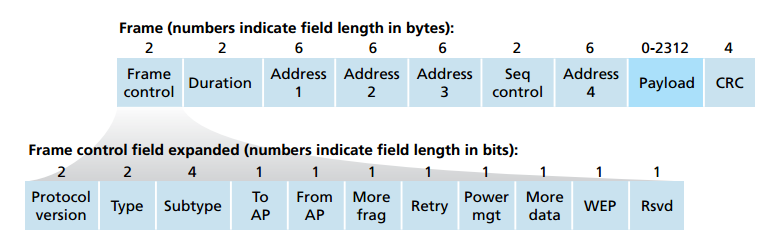
\includegraphics[width=\linewidth]{images/trama-wifi.png}
    \caption{Estructura de una trama \emph{WiFi} \autocite{Kurose:Wireless}}
\end{figure}

\begin{itemize}
    \item PDU (\emph{Payload}): datos que lleva la trama, mayormente es un datagrama IP o un paquete ARP. Puede ser de hasta 2312 bytes pero habitualmente es menor o igual a 1500 bytes
    \item CRC (\emph{Cyclic Redundancy Check}): palabra de 32 bits que sirve para detectar errores en el receptor.
    \item Direcciones: una trama 802.11 puede llevar hasta \emph{cuatro direcciones MAC} (tres son necesarias para transferir un datagrama de capa de red desde una terminal inalámbrica hasta la interfaz de un router, a través de un AP; la cuarta dirección es para trabajar en modo \emph{Ad Hoc}).
    \begin{itemize}
        \item Dirección 1: dirección MAC del receptor
        \item Dirección 2: dirección MAC del emisor
        \item Dirección 3: dirección MAC de la interfaz del router que forma parte del \emph{BSS} 
    \end{itemize}
    \item Número de secuencia: enumeración de los bytes enviados en cada trama; tiene la misma funcionalidad que el número de secuencia en TCP.
    \item Duración: cuando un nodo está transmitiendo datos por un canal, tiene reservado el canal por un tiempo determinado. Este campo de duración indica ese valor.
    \item Campos de control:
    \begin{itemize}
        \item \emph{Versión del protocolo}
        \item \emph{Tipo} y \emph{subtipo:} distinguen si la trama es para una petición/respuesta de asociación, si es RTS/CTS, un ACK, o una trama con datos.
        \item \emph{Hacia AP} y \emph{desde AP}: definen el \emph{significado} de los diferentes campos de dirección (pueden cambiar si se trabaja en modo \emph{infraestructura} o en modo \emph{Ad Hoc})
        \item \emph{More frag}: indica si vienen fragmentos después de la trama. 
        \item \emph{Retry}: indica si es una retransmisión 
        \item \emph{Power Management}: indica si la estación está en modo \emph{ahorro de energía}.  
        \item \emph{More data}: indica si el AP tiene datos en un buffer que están destinados para una estación que está en modo \emph{ahorro de energía}.  
        \item \emph{WEP}: indica si se está utilizando o no la el algoritmo \emph{WEP} para encriptar los datos de la trama.
        \item \emph{Rsvd}: indica si la transmisión tiene alguna restricción. 
    \end{itemize}

\end{itemize}






















%%%%%%%%%%%%%%%%%%%%%%%%%%%%%%%%%%%%%%%%%%%%
% FIN DOCUMENTO, AHORA REFERENCIAS
%%%%%%%%%%%%%%%%%%%%%%%%%%%%%%%%%%%%%%%%%%%%
\clearpage
\printbibliography

\end{document}

